\documentclass[12pt]{article}

\usepackage{alltt}
\usepackage{epsfig}
\usepackage{pstricks}
\usepackage{xspace}
\usepackage{url}
%\usepackage{makeidx}
%\usepackage{index}
%\usepackage{multind}

%\makeindex

%\newindex{MLbn}{bnx}{bnd}{Index of ML bindings}
%\newindex{MLty}{tnx}{tnd}{Index of ML types}

\newcommand{\bnind}[1]{\index[MLbn]{#1}}
\newcommand{\tyind}[1]{\index[MLty]{#1}}


\newlength{\minipagewidth}
\setlength{\minipagewidth}{\textwidth}
\addtolength{\minipagewidth}{-5mm}

\newenvironment{greekenumerate}{\begin{enumerate}
  \renewcommand{\theenumi}{\roman{enumi}}
  \renewcommand{\labelenumi}{(\roman{enumi})}}{\end{enumerate}}

\renewcommand{\t}[1]{\mbox{\small\tt #1}}
\newcommand{\con}[1]{\mbox{\sf #1}}
\newcommand{\ty}[1]{\mbox{\tt #1}}
\newcommand{\prev}[1]{#1}

\newcommand{\varord}[1]{#1}

\newcommand{\ma}[1]{{{$#1$}}}
\newcommand{\ml}[1]{{\tt #1}}
\newcommand{\id}[1]{#1}

\newcommand{\redonlightgray}[1]%
{\psset{fillcolor=lightgray}\psframebox*[framearc=.3]{\red #1}}

\newcommand\HOL{HOL\xspace}
\newcommand\Hol{Hol98\xspace}
\newcommand{\mosml}{Moscow~ML\xspace}
\newcommand{\Buddy}{BuDDy\xspace}
\newcommand{\Muddy}{MuDDy\xspace}
\newcommand\HolBuddy{{Hol98{+}\Buddy\xspace}}

\newcommand\fun{\mbox{\tt{->}}}
\newcommand\turn{{\vdash}}
\newcommand\imp{{\Rightarrow}}
\newcommand\T{\con{T}}
\newcommand\F{\con{F}}

\newcommand{\cond}{\rightarrow}
\newcommand{\els}{\mid}
\newcommand{\Imp}{\Rightarrow}

\renewcommand{\prod}{\mbox{\tt{*}}}
\newcommand{\SP}{~}
\newcommand{\SPP}{~}

\newcommand{\homedir}{\mbox{$\sim$}}

\newcommand{\Turn}{\(\turn\)}
\newcommand{\And}{\(\wedge\)}
\newcommand{\Or}{\(\vee\)}
\newcommand{\Not}{\(\neg\)}
\newcommand{\Forall}{\(\forall\)}
\newcommand{\Exists}{\(\exists\)}
\newcommand{\Mapsto}{\(\mapsto\)}


\parindent 0mm
\parskip 1mm


% ---------------------------------------------------------------------
% Macros for little HOL sessions displayed in boxes.
%
%	     \begin{session}\begin{verbatim}
%	      .
%	       < lines from hol session >
%	      .
%	     \end{verbatim}\end{session}   
%
%            typesets the session in a box.
% ---------------------------------------------------------------------

\newlength{\hsbw}
\setlength{\hsbw}{\textwidth}
\addtolength{\hsbw}{-\arrayrulewidth}
\addtolength{\hsbw}{-\tabcolsep}

\newcommand\MLSpacing{13pt}
\newenvironment{session}{\begin{flushleft}
 \begin{tabular}{@{}|c@{}|@{}}\hline 
 \begin{minipage}[b]{\hsbw}
 \begingroup\small\baselineskip\MLSpacing}{\endgroup\end{minipage}\\ \hline 
 \end{tabular}
 \end{flushleft}}

\begin{document}
\thispagestyle{empty}

\hrule height5pt

\begin{flushleft}\Huge
{\tt HolSatLib} Documentation\\
{\Large Version 1.0$\beta$}
\end{flushleft}

\vspace*{2mm}

\hrule height5pt

\vspace*{1cm}


\noindent{\Large{\bf Mike Gordon}}

\vspace*{5mm}

\today

\vfill

{\setlength{\fboxrule}{0.5mm}
\setlength{\fboxsep}{2mm}
\fbox{
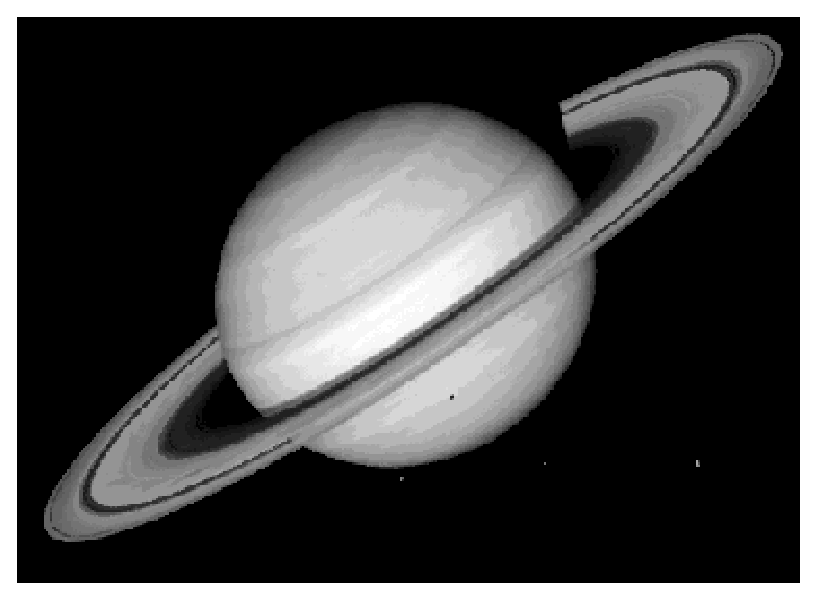
\epsfig{file=saturn.ps}% \raisebox{2.5cm}{\Huge\bf~~~+~} 
}}

\vfill

\newpage

\pagenumbering{roman}

\section*{Preface}



This document describes {\tt{HolSatLib}}
as distributed with the {\it Kananaskis\/} release of Hol98. Section~\ref{install}
describes how to install it with {\it Taupo} releases.

{\tt{HolSatLib}} provides a very simple harness in Hol98 for
invoking SAT solvers on \HOL terms. Currently the following
solvers are supported

\medskip

\begin{tabular}{ll}
{\bf Solver} & {\bf Home Page} \\ \hline
SATO & {\small\url{http://www.cs.uiowa.edu/~hzhang/sato.html}}\\
GRASP & {\small\url{http://sat.inesc.pt/~jpms/grasp}}\\
ZCHAFF & {\small\url{http://www.ee.princeton.edu/~chaff/zchaff.html}}
\end{tabular}

\medskip

These solvers all require input in the standard DIMACS 
format\footnote{\small\tt ftp://dimacs.rutgers.edu/pub/challenge/satisfiability/}
for conjunctive normal form (CNF). It should be straightforward to add other
DIMACS compatible SAT solvers.

The purpose of {\tt{HolSatLib}} is to provide a platform
for experimenting with combinations of theorem proving and
SAT. Hol98 can be used to deductively manipulate terms into CNF as
required for SAT analysis, and then the results of the analysis
can be reimported into \HOL and either checked or just trusted.

Currently {\tt
HolSatLib} has only been tested under Linux, though it should be
possible to run it under Windows.





\vfill

\begin{flushright}
Mike Gordon\\
\today
\end{flushright}


\newpage

{\baselineskip10pt
\tableofcontents
}

\newpage
\pagenumbering{arabic}

\section{Introduction}


The following examples illustrates {\tt{HolSatLib}} in action.

\begin{session}\begin{verbatim}

- load "HolSatLib"; open HolSatLib
[ output omitted ]
> val it = () : unit

- show_tags := true;
> val it = () : unit

- satOracle grasp ``(x \/ ~y \/ z) /\ (~z \/ y)``;
> val it = [oracles: grasp] [axioms: ] [] 
           |- z /\ y ==> (x \/ ~y \/ z) /\ (~z \/ y) : thm

- satProve grasp ``(x \/ ~y \/ z) /\ (~z \/ y)``;
> val it = [oracles: ] [axioms: ] [] 
           |- z /\ y ==> (x \/ ~y \/ z) /\ (~z \/ y) : thm

\end{verbatim}\end{session}

Setting \t{show\_tags} to \t{true} makes the \Hol top
level print theorem tags.

The function \t{satOracle} takes a SAT solver (currently either
\t{sato}, \t{grasp} or \t{zchaff}, but more could be added) and a term
$t$ and

\begin{enumerate}
\item writes a DIMACS format file corresponding to the term $t$
\item invokes the solver on the file to create an output file
\item parses the output file to extract the model found
\item creates a theorem, tagged with the name of the solver, that shows the model.
\end{enumerate}

The function \t{satProve} performs steps 1--3 above, but then uses
\Hol to check that the model is really a model and then
returns an untagged theorem. Note that checking a model is
generally much quicker than finding it (one just `evaluates' the term
with the values supplied by the model).

Thus if one is prepared to trust the solver then use \t{satOracle},
but if one wants to verify the results (which could be time-consuming)
use \t{satProve}.


The next example illustrates what happens on unsatisfiable terms.

\begin{session}\begin{verbatim}

- satOracle grasp ``(x \/ ~y \/ z) /\ ~z /\ y /\ ~x``;
> val it = [oracles: grasp] [axioms: ] [] 
           |- ~((x \/ ~y \/ z) /\ ~z /\ y /\ ~x)

- satProve grasp ``(x \/ ~y \/ z) /\ ~z /\ y /\ ~x``;
! Uncaught exception: 
! satProveError

\end{verbatim}\end{session}

If a term $t$ is unsatisfiable then \t{satOracle} will return {\small\verb+|- ~+}$t$,
tagged with the name of the SAT solver used. However, \t{satProve} will raise an exception,
since there is no efficient way to check for unsatisfiability using pure \Hol
theorem proving.

A tautology checker that uses SAT can be easily programmed using
\t{CNF\_CONV}, which is supplied in the structure \t{canonTools} that comes
with \t{HolSatLib}. To check the validity of a term $t$

\begin{quote}
\begin{description}
\item[\t{[th1]}] use \t{CNF\_CONV} to prove {\small\verb+|- ~+}$t~=~t'$, where $t'$ is in CNF;
\item[\t{[th2]}] use SAT to prove  {\small\verb+|- ~+}$t'$;
\item[\t{[th3]}] by negating both sides of \t{th1}, prove {\small\verb+|- ~~+}$t~=~{\small\verb+~+}t'$;
\item[\t{[th4]}] hence by combining \t{th2} and \t{th3} derive {\small\verb+|- ~~+}$t$.
\item[\t{[th5]}] hence by the law of double negation conclude {\small\verb+|- +}$t$.
\end{description}
\end{quote}

Example \Hol code to mechanise these steps is as follows:

\begin{session}\begin{verbatim}

(* NOT_CLAUSES = |- (!t. ~~t = t) /\ (~T = F) /\ (~F = T)  *)
val NOT_NOT = CONJUNCT1 NOT_CLAUSES;

fun SAT_TAUT_CHECK sat_solver t =
 let val th1 = canonTools.CNF_CONV(mk_neg t)
     val th2 = satOracle sat_solver (rhs(concl th1))
     val th3 = AP_TERM ``$~`` th1
     val th4 = EQ_MP (SYM th3) th2
     val th5 = EQ_MP (SPEC t NOT_NOT) th4
 in
  th5
 end;

\end{verbatim}\end{session}

\section{Installing {\tt HolSatLib} under Linux}\label{install}

\begin{enumerate}

\item Visit \url{http://www.cl.cam.ac.uk/~mjcg/HolSatLib} and
download the file {\tt HolSatLib.tar.gz}

\item place  {\tt HolSatLib.tar.gz} in a directory {\it dir}
(where {\it dir} is an absolute path name)

\item connect to {\it dir} and execute\\[-9mm]
{\small\begin{verbatim}
   gunzip HolSatLib.tar.gz; tar -xf HolSatLib.tar
\end{verbatim}}
\vspace*{-4mm}
this should result in a directory {\it dir}{\tt/HolSatLib} containing
\vspace*{-4mm}
{\small\begin{verbatim}
   Cnf.sml HolSatLib.sig HolSatLib.sml SatSolvers.sml doc sat_solvers
\end{verbatim}}

\item connect to {\it dir}{\tt/HolSatLib} and execute\\[-9mm]
{\small\begin{verbatim}
   Holmake cleanAll; Holmake
\end{verbatim}}
\vspace*{-4mm}
you should see
\vspace*{-4mm}
{\small\begin{verbatim}
   Analysing HolSatLib.sml
   Trying to create directory .HOLMK for dependency files
   Analysing HolSatLib.sig
   Compiling HolSatLib.sig
   Analysing SatSolvers.sml
   Compiling SatSolvers.sml
   Compiling HolSatLib.sml
   Analysing Cnf.sml
   Compiling Cnf.sml
\end{verbatim}}

\item download SATO, GRASP and ZCHAFF into the directories {\tt sato}, {\tt grasp},
{\tt zchaff}, respectively, in {\it dir}{\tt/HolSatLib/sat\_solvers}
(versions may already be there)

\item after starting \Hol execute\\[-9mm]
{\small\begin{alltt}
   loadPath := "\({\it{dir}}\)/HolSatLib" :: !loadPath;
\end{alltt}}

\item you should now be able to execute\\[-9mm]
{\small\begin{verbatim}
   load "HolSatLib"; open HolSatLib;
\end{verbatim}}
\end{enumerate}

\section{{\tt HolSatLib} Documentation}

{\tt HolSatLib} currently comes with three
modules


\medskip

\begin{tabular}{ll}
{\bf Module} & {\bf Description} \\ \hline
{\tt HolSatLib} & functions for invoking SAT solvers\\
{\tt SatSolvers} & specifications of \t{sato}, \t{grasp} and \t{zchaff}\\
{\tt Cnf} & tool for converting \HOL terms to CNF (from Joe Hurd)
\end{tabular}

\medskip

\subsection{Contents of {\tt HolSatLib} module}

The signature of {\tt HolSatLib} is shown below, followed
by a description of the components.

{\small\begin{verbatim}
signature HolSatLib = sig
  datatype sat_solver = 
   SatSolver of {name           : string,
                 URL            : string,
                 executable     : string,    
                 notime_run     : string -> string * string -> string,    
                 time_run       : string -> (string * string) * int -> string,      
                 only_true      : bool,
                 failure_string : string,
                 start_string   : string,  
                 end_string     : string}
  val sato          : sat_solver
  val grasp         : sat_solver
  val zchaff        : sat_solver
  val tmp_name      : string ref
  val sat_command   : string ref
  val prefix        : string ref
  val showSatVarMap : unit -> int * (string * int) list
  val satOracle     : sat_solver -> Term.term -> Thm.th
  val satProve      : sat_solver -> Term.term -> Thm.thm
  val readDimacs    : string -> Term.term
\end{verbatim}}

\subsubsection{\tt sat\_solver}

The datatype \t{sat\_solver} is defined in the module {SatSolvers}.
The data in the record argument to the constructor \t{SatSolver}
is an ad-hoc list of what is needed to invoke a SAT program
and parse the results. One only needs to know what the fields
contain if one is adding another SAT prover. See the
source code {\tt SatSolvers.sml} for some information
in the comments.

\subsubsection{{\tt sato}, {\tt grasp} and {\tt zchaff}}

The ML identifiers \t{sato}, \t{grasp} and \t{zchaff} are bound
by module {\tt SatSolvers} to descriptions of the corresponding SAT solvers.
These descriptions are passed to \t{satOracle} and \t{satProve} to
select which SAT solver to invoke.

\subsubsection{{\tt tmp\_name}, {\tt sat\_command}, {\tt prefix} and {\tt showSatVarMap}}

The reference \t{tmp\_name} contains the temporary file name used in
the last invokation of a SAT solver  by \t{satOracle} or \t{satProve}. This name
was generated using \t{FileSys.tmpName}.



The reference \t{sat\_command} contains the actual command executed
(using \t{Process.system}) for
the last invokation of a SAT solver. This command reads from
an input file and writes to an output file. The file names are generated by extending \t{tmp\_name}
(the input file name extension is \t{cnf} and the out extension is the name of the SAT solver used).


The reference \t{prefix} contains the string that is concatenated to numbers
to get the \HOL variables used when reading a separately generated DIMACS file
with \t{readDimacs}. Default value is {\verb+"v"+}.

The function {\small\verb+showSatVarMap+} returns a pair consisting of
the one plus the number of variables used (i.e. the first number not
currently used as a variable) and the mapping from variable names to
numbers for encoding a term in DIMACS format by
\t{satOracle} or \t{satProve}.


\subsubsection{\tt satOracle}

{\small{\tt satOracle}~{\it solver}~{\it term}}


\begin{enumerate}
\item writes a DIMACS format file corresponding to {\it term}
\begin{enumerate}
\item the mapping from \HOL variable names to integers can be seen using
\t{showSatVarMap}
\item the input file name is {\it tmp}{\tt{.cnf}}, where
the string {\it tmp} is in the reference \t{tmp\_name}
\end{enumerate}


\item invokes {\it solver} on the file and writes results to an output file


\begin{enumerate}
\item the default settings (time, verbosity etc.) supplied by {\it solver}
are used
\item the output file name is {\it tmp}{\tt{.}}{\it{name}}, where
the string {\it tmp} is in the reference \t{tmp\_name}
and {\it name} is the string given as the value of the field {\tt name} of {\it solver}
\item the actual command executed can be seen in the reference 
\t{sat\_command}
\end{enumerate}


\item parses the output file to see if a model was found and if so extracts it


\begin{enumerate}
\item the presence of the string given as the value of the
field {\tt failure\_string} in {\it solver} is
assumed to indicate that {\it term} is unsatisfiable
\item if {\it term} is not unsatisfiable,
the model is assumed to be supplied as a list of integers in the output file 
{\it tmp}{\tt{.}}{\it{name}} between the strings
given as the values of the fields {\tt start\_string} and {\tt end\_string}
in {\it solver}
\item the mapping available via \t{showSatVarMap} is used
to turn the extracted model into a \HOL term
\item if the value of the field {\tt only\_true} is
\t{true} then it is assumed that only the positive literals
of the model are given (this is the case with SATO) and so
the negative literals are taken to be the negations of those variables
occurring in {\it term}, but not in the computed model
\end{enumerate}


\item creates a theorem, tagged with the name of {\it solver}, showing the result

\begin{enumerate}

\item if {\it term} is unsatisfiable the result is the tagged theorem {\small\verb+|- ~+}{\it{term}}
\item if a model is found the result is the tagged theorem 
{\small\verb+|- +}{\it{model}}{\small\verb+ ==> +}{\it{term}},
where {\it model} is the conjunction of the literals extracted from the model
\item the oracle tag is the name of {\it solver}.
\end{enumerate}
\end{enumerate}

\subsubsection{\tt satProve}

{\small{\tt satProve}~{\it solver}~{\it term}} goes through the same steps 1,2 and 3 
as {\tt satOracle}, but instead of step 4

\begin{enumerate}
\item  if
a model is found, then proof in \Hol is used to first check the model
is really a model (by `evaluating' {\it term} using the model) and if it
is an untagged theorem {\small\verb+|- +}{\it{model}}{\small\verb+ ==> +}{\it{term}}
is returned

\item if a model is found by {\it solver}, but the \Hol check fails, 
i.e.~the model is invalid, then the exception \t{satProveError} is raised

\item if {\it term} is found to be unsatisfiable by {\it solver},
the exception \t{satProveError} is raised

\end{enumerate}

\subsubsection{\tt readDimacs}

{\small{\tt readDimacs}~{\it file}} reads a DIMACS format file and returns
an CNF \HOL term corresponding the the SAT problem in the file names {\it file}.
The integers in the file are prefixed with the string in the reference 
\t{prefix} (the default is {\small\verb+"v"+}).

{\small{\tt readDimacs}} is mainly intended as a tool for getting
CNF examples by reading in examples from the DIMACS problem set,
which is distributed with {\tt HolSatLib} in the directory
{\tt HolSatLib/doc/DIMACS} or is available from\\
{\tt ftp://dimacs.rutgers.edu/pub/challenge/satisfiability/benchmarks/cnf/}.

\subsection{Contents of {\tt SatSolvers} module}

{\tt SatSolvers} contains the definition of the datatype
\t{sat\_solver} for specifying SAT solvers.


The record that is supplied as an argument to the constructor \t{SatSolver}
has the following fields.

\medskip

\begin{tabular}{ll}
\t{name} &
name of the SAT solver \\

\t{URL} &
URL of the SAT executable for downloading\\

\t{executable} &
name of the SAT solver command\\

\t{notime\_run} &
evaluating \t{notime\_run}{\it~ex~(infile,outfile)} returns a string\\
 & giving a command to execute to run the SAT solver from input\\
 & {\it infile} and produce output {\it outfile}; the paramenter\\
 & {\it ex} should be the full path name of the  SAT solver command\\
 & all command options are the defaults (see solver documentation)\\

\t{time\_run} &
evaluating \t{time\_run}{\it~ex~((infile,outfile),time)} returns a string\\
 & giving a command to execute to run the SAT solver for {\it time} units\\
 & of time (the units are specified in the SAT solver's documentation)\\
 & from input {\it infile} and produce output {\it outfile}; the paramenter\\
 & {\it ex} should be the full path name of the  SAT solver command;\\
 & all command options, besides the time, are the defaults\\
 & (currently \t{time\_run} is not used)\\

\t{failure\_string} &
string whose presence in the solver output indicated unsatisfiability\\


\t{start\_string} &
string indicating start of model \\


\t{end\_string} &
string indicating end of model \\

\end{tabular}

\medskip

Note that if a model is found, it is assumed to be bracketed
by \t{start\_string} and \t{end\_string}. SAT solvers 
(like {\tt satz}\footnote{\url{http://www.laria.u-picardie.fr/~cli/EnglishPage.html}})
for which models are not bracketed by a fixed pair of strings cannot currently
be specified for use with {\tt HolSatLib}. If access to such solvers is needed, then
it will be necessary to extend the datatype \t{sat\_solver} to contain
additional parsing data (e.g.~regular expressions).

\subsection{Contents of {\tt canonTools} module}

The module {\tt canonTools} contains a simple conversion 
{\small\verb+CNF_CONV : term -> thm+}, 
from Joe Hurd, to convert
\HOL terms to a form suitable for inputting to \t{satOracle} or \t{satProve}.

{\small\verb+CNF_CONV+}~$t$ returns a theorem {\small\verb+|- +}$t\t{~=~}t'$,
where $t'$ is in CNF.

There are other tools for converting to various canonical forms. See the source code
{\small\verb+canonTools.sml+} for details.

\end{document}
